\chapter{NLP2RDF}

\emph{NLP2RDF}\footnote{Webseite \url{http://nlp2rdf.org}, Download (Open Source) unter \url{http://code.google.com/p/nlp2rdf}}
ist ein Framework, das viele verschiedene Tools zur Verarbeitung natürlicher Sprache (\emph{natural-language processing, NLP}) integriert.
NLP2RDF verarbeitet geschriebene Sätze und wandelt diese in eine RDF-Struktur um, die mit syntaktischen und semantischen Zusatzinformationen angereichert ist.
\begin{figure}[htb]
\begin{center}
\begin{threeparttable}
\includegraphics[width=0.5\textwidth]{img/nlp2rdf_stack.png}
\begin{tablenotes}\footnotesize
 \item [] Quelle: \citet{tiger_corpus_navigator}
\end{tablenotes}
\end{threeparttable}
\caption{Der \emph{NLP2RDF stack}}
\label{fig:nlp2rdf_stack}
\end{center}
\end{figure}
Dabei werden die Sätze zunächst durch einen Chunker in Tokens zerlegt, aus denen ein Grundgerüst erstellt wird, die \emph{Structured Sentence ontology (SSO)}.
Die SSO besteht nur aus einem minimalen Vokabular und der grundlegenden Struktur des Satzes in Form der Tokens und ihrer Position im Satz, siehe Abbildung \ref{fig:nlp2rdf_sso}.
Nun werden schrittweise Zusatzinformationen hinzugefügt.
Im ersten Schritt sind dies Features aus NLP-Verfahren (türkis bzw. hellgrau in Abbildung \ref{fig:nlp2rdf_stack}), im zweiten Schritt Ontologien für diese Features.
Dem Wort "`wir"' eines Satzes könnte also im ersten Schritt das Feature "`ist ein Personalpronomen"' zugeordnet werden und dem Wort "`unser"' eines anderen Satzes das Feature "`ist ein Possessivpronomen"'.
Enthält nun die Ontologie die Klassenbeziehungen "`ein Personalpronomen ist ein Pronomen"' und "`ein Personalpronomen ist ein Pronomen"', dann macht dies die Aussage
"`beide Sätze enthalten ein Pronomen"' möglich, was wiederum weitere Schlussfolgerungen auf komplexere Features ermöglicht.
Im dritten Schritt wird nun eine \emph{Wortsinndisambiguierung} (im Folgenden auch nur \emph{Disambiguierung} oder \emph{WSD}, eine Mehrdeutigkeitsauflösung) durchgeführt und Hintergrundwissen aus dem Semantischen Web (rot bzw. dunkelgrau) hinzugefügt.
Im Satz "`Er war ein echter Berliner und fühlte sich in seiner Stadt pudelwohl."' würde beispielsweise die Disambiguierung festlegen, dass sich das Wort "`Berliner"' nicht auf den \emph{Berliner Pfannkuchen} sondern auf
die Stadt \emph{Berlin} bezieht, worauf nun weitere Informationen über diese Stadt in die Struktur integriert werden könnten, \zb{} die Einwohnerzahl und geographische Lage der Stadt Berlin.
%Im Satz "`Er kaufte sich einen Pfannkuchen mit einer Füllung aus Konfitüre"' 

%\paragraph{Ein Beispiel}

\begin{figure}
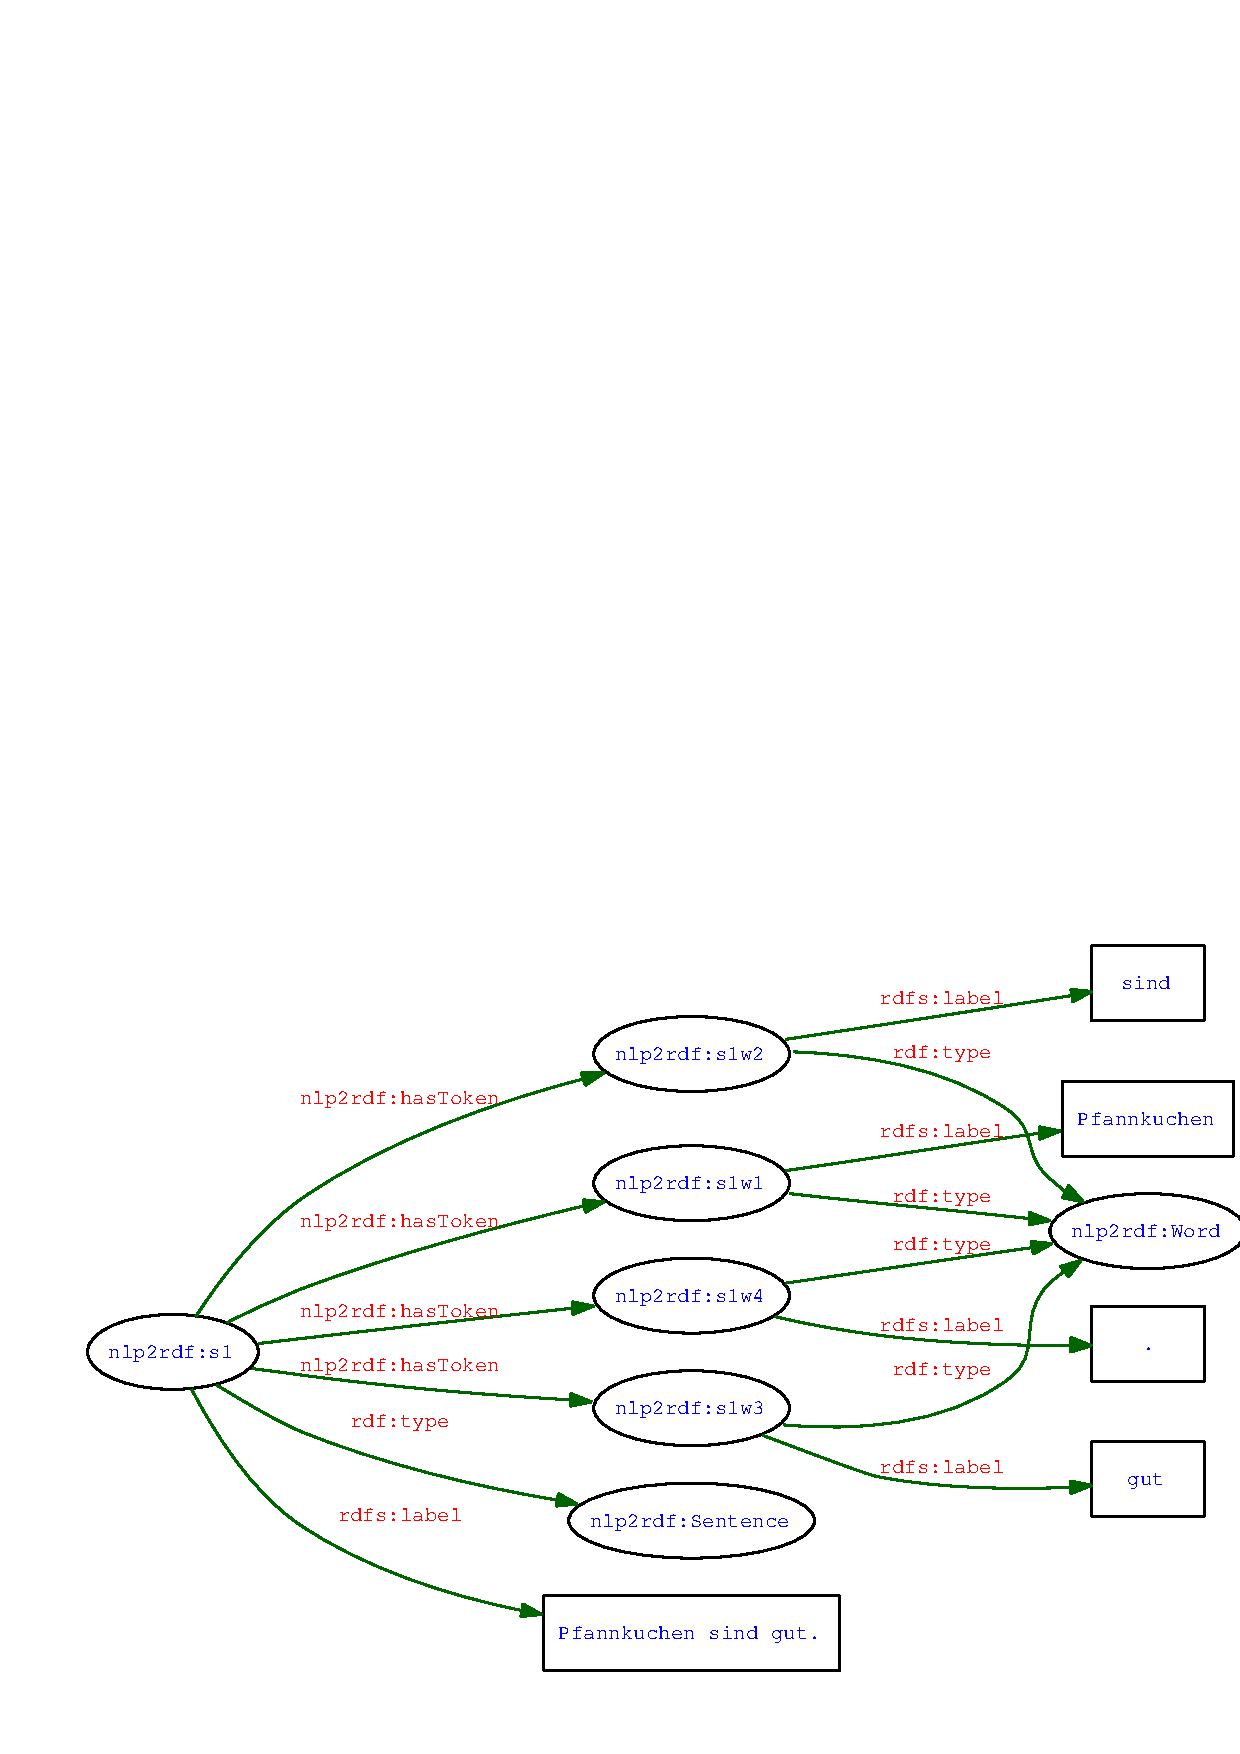
\includegraphics[width=\textwidth]{img/pdf/sso.pdf}
\caption{die \emph{Sentence Structure ontology} eines Beispielsatzes}
\label{fig:nlp2rdf_sso}
\end{figure}
%\footnote{\url{http://www.w3.org/RDF/Validator/}}
\iffalse
\lstset{language=XML}
\begin{lstlisting}
<?xml version="1.0"?>
<rdf:RDF xmlns:rdf="http://www.w3.org/1999/02/22-rdf-syntax-ns#"
    xmlns="http://nlp2rdf.org/"
    xmlns:ns0="http://www.w3.org/2002/07/owl#"
    xmlns:dcterms="http://purl.org/dc/terms/"
    xmlns:xsd="http://www.w3.org/2001/XMLSchema#"
    xmlns:j.0="http://141.89.100.105/owl/stts.owl#"
    xmlns:j.1="http://www.w3.org/2000/01/rdf-schema#" > 
 
  <rdf:Description rdf:about="http://nlp2rdf.org/s1">
    <hasWord rdf:resource="http://nlp2rdf.org/s1w1"/>
    <hasWord rdf:resource="http://nlp2rdf.org/s1w2"/>
    <hasWord rdf:resource="http://nlp2rdf.org/s1w3"/>
    <hasWord rdf:resource="http://nlp2rdf.org/s1w4"/>
    <rdf:type rdf:resource="http://nlp2rdf.org/Sentence"/>
    <j.1:label>Pfannkuchen sind gut.</j.1:label>
  </rdf:Description>
 <rdf:Description rdf:about="http://nlp2rdf.org/s1w1">
    <j.1:label>Pfannkuchen</j.1:label>
    <rdf:type rdf:resource="http://nlp2rdf.org/Word"/>
  </rdf:Description>
 <rdf:Description rdf:about="http://nlp2rdf.org/s1w2">
    <j.1:label>sind</j.1:label>
    <rdf:type rdf:resource="http://nlp2rdf.org/Word"/>
  </rdf:Description>
 <rdf:Description rdf:about="http://nlp2rdf.org/s1w3">
    <j.1:label>gut</j.1:label>
    <rdf:type rdf:resource="http://nlp2rdf.org/Word"/>
  </rdf:Description>
 <rdf:Description rdf:about="http://nlp2rdf.org/s1w4">
    <j.1:label>.</j.1:label>
    <rdf:type rdf:resource="http://nlp2rdf.org/Word"/>
  </rdf:Description>
</rdf:RDF>
\end{lstlisting}
\lstset{language=Java}
\fi
\iffalse
das hier für die visualisierung benutzen (rdf:x durch rdf1:x ersetzen), damit die abkürzungen reinkommen statt der vollen uri
    <?xml version="1.0"?>
<rdf:RDF
    xmlns:rdf="http://www.w3.org/1999/02/22-rdf-syntax-ns#"
    xmlns:rdf1="rdf:"
    xmlns:nlp2rdf="nlp2rdf:"
    xmlns="nlp2rdf:"
    xmlns:ns0="owl:"
    xmlns:dcterms="dcterms:"
    xmlns:xsd="xsd:"
    xmlns:j.0="stts:"
    xmlns:j.1="rdfs:" > 
 
  <rdf:Description rdf:about="nlp2rdf:s1">
    <hasToken rdf:resource="nlp2rdf:s1w1"/>
    <hasToken rdf:resource="nlp2rdf:s1w2"/>
    <hasToken rdf:resource="nlp2rdf:s1w3"/>
    <hasToken rdf:resource="nlp2rdf:s1w4"/>
    <rdf1:type rdf:resource="nlp2rdf:Sentence"/>
    <j.1:label>Pfannkuchen sind gut.</j.1:label>
  </rdf:Description>
 <rdf:Description rdf:about="nlp2rdf:s1w1">
    <j.1:label>Pfannkuchen</j.1:label>
    <rdf1:type rdf:resource="nlp2rdf:Word"/>
  </rdf:Description>
 <rdf:Description rdf:about="nlp2rdf:s1w2">
    <j.1:label>sind</j.1:label>
    <rdf1:type rdf:resource="nlp2rdf:Word"/>
  </rdf:Description>
 <rdf:Description rdf:about="nlp2rdf:s1w3">
    <j.1:label>gut</j.1:label>
    <rdf1:type rdf:resource="nlp2rdf:Word"/>
  </rdf:Description>
 <rdf:Description rdf:about="nlp2rdf:s1w4">
    <j.1:label>.</j.1:label>
    <rdf1:type rdf:resource="nlp2rdf:Word"/>
  </rdf:Description>
</rdf:RDF>
\fi

\section{Der Parser}
Die Morphologie und die \emph{Part of Speech} (POS) \emph{Tags} eines Eingabesatzes werden von einem Parser bestimmt.
%Diese Struktur wird dann in RDF modelliert und wie ein Weihnachtsbaum von beliebigen weiteren Tools mit Zusatzinformationen behängt.

%\begin{floatingfigure}[r]{0.5\textwidth}
\begin{figure}[0.5\textwidth]
    %\centering
    \includegraphics[width=0.5\textwidth]{img/stts_ontology_alpha.png}
    \caption{die angepasste STTS-Ontologie (frühe Version)}
    \label{fig:stts_ontology_alpha}
\end{figure}
%\end{floatingfigure}

Dabei wird der statistische Parser der Stanford Natural Language Group\footnote{\url{http://nlp.stanford.edu/software/lex-parser.shtml}} benutzt, aufgrund der modularen Struktur von NLP2RDF
sind andere Parser aber auch problemlos einbindbar.
Für nichtkommerzielle Nutzung ist er frei verfügbar und als Javaprogramm leicht integrierbar.
Ein trainiertes Modell ist unter anderem für Deutsch und Englisch bereits enthalten.

%Um den Output des Parsers in eine RDF-Struktur zu übertragen, ist eine passende Ontologie nötig, welche die Relation der Annotierungen untereinander festlegt (\zb{} "`Ein Reflexivpronomen ist ein Pronomen"').
Da der deutsche Parser\footnote{germanFactored.ser.gz} auf dem Negra Corpus\footnote{\url{http://www.coli.uni-saarland.de/projects/sfb378/negra-corpus/negra-corpus.html}} basiert,
 welches das Stuttgart-Tübingen Tagset (STTS)\footnote{\url{http://www.sfs.uni-tuebingen.de/Elwis/stts/stts.html}} benutzt,
kann eine bereits existierende STTS-Ontologie\footnote{\url{http://141.89.100.105/owl-docu/stts.html}} mit kleineren Erweiterungen direkt benutzt werden (siehe Abbildung \ref{fig:stts_ontology_alpha}).

Die mitgelieferten englischen Parser\footnote{englishFactored.ser.gz und englishPCFG.ser.gz} benutzen die Tags des Penn Treebank Projektes\footnote{\url{http://www.cis.upenn.edu/~treebank/}} -- das Penn Treebank Tag Set.
Eine passende Ontologie wird freundlicherweise von Herrn Christian Chiarcos\footnote{Arbeitsseite: \url{http://www.sfb632.uni-potsdam.de/~chiarcos/}} zur Verfügung gestellt.
Sie wurde im Rahmen des Projektes “Sustainability of Linguistic Data” an der Universität Potsdam entwickelt und gehört zu einem integrativen Framework \citep{ontology-based_interface_specifications}.

\iffalse
%
\iffalse
Unglücklicherweise konnte keine Ontologie für das Penn Treebank Tag Set gefunden werden. Aufgrund des bereits großen Umfanges dieser Arbeit und des Umstandes, das der Autor kein ausgebildeter Sprachwissenschaftler ist,
 erschien es auch nicht praktikabel, solch eine Ontologie selbst zu erstellen.
Das Umlernen eines POS-Taggers auf ein anderes Tagset ist beim Stanford Parser jedoch möglich, wenn man ihn mit POS-annotierten Trainingstexten versorgt.\footnote{\url{http://nlp.stanford.edu/software/parser-faq.shtml#f}}
Es war also nur noch eine beliebige für das Englische geeignete Ontologie gesucht, für die es POS-annotierten Text gibt.
Die Wahl fiel dabei auf das Susanne\footnote{Surface and underlying structural analysis of natural English}-Tagset.
Sowohl das Susanne Corpus, eine passende Treebank\footnote{\url{www.grsampson.net/Resources.html}} als auch die Ontologie\footnote{\url{http://141.89.100.105/owl-docu/susa.html}} sind frei verfügbar.

In der FAQ des Stanford Parsers wird ein Satz angegeben, der das erwartete Format deutlich macht:

\begin{verbatim}
`The/DT quick/JJ brown/JJ fox/NN jumped/VBD over/IN the/DT lazy/JJ dog/NN ./.
\end{verbatim}

Die Treebank besteht jedoch aus mehreren Dateien, welche Zeilen wie diese enhalten:
\begin{verbatim}
G12:0030.27	-	PPHS1m	He	he	[S[Nas:s.Nas:s]
G12:0030.30	-	VBDZ	was	be	[Vsu.
G12:0030.33	-	VVGv	waiting	wait	.Vsu]S]
G12:0030.39	-	YF	+.	-	.O]
\end{verbatim}
Das gewünschte Format kann daraus jedoch erzeugt werden.

Zusammenführen aller relevanten Dateien in Eine:
\begin{verbatim}
find | sed "s/\.\///" |
egrep -v "lexicon|documentation|\." |
xargs cat >>allinone.txt
\end{verbatim}
Auswählen der relevanten Spalten:
\begin{verbatim}
cat allinone.txt | cut -f3,4 > allinone_tag_and_word.csv
\end{verbatim}
Vertauschen der Spalten und Einsetzen des Trennzeichens:
\begin{verbatim}
cat allinone_tag_and_word.csv |
sed "s/\([^\t]*\)\t\([^\t]*\)/\2\/\1/"
> allinone_stanfordformat.txt
\end{verbatim}
Alle Zeilenumbrüche entfernen:
\begin{verbatim}
cat allinone_stanfordformat.txt |
tr "\n" " " > allinone_stanfordformat_oneline.txt
\end{verbatim}
Zeilenumbrüche nach dem Satzende hinzufügen um das endgültige Format zu bekommen:
\begin{verbatim}
cat allinone_stanfordformat_oneline.txt |
sed "s/+\.\/YF /+\.\/YF\\n/g"
> susanne_treebank_readyfortraining.txt
\end{verbatim}
\todo{was ist mit einem trainierten parser model für die susa.owl?}
\todo{was ist mit einem trainierten parser model für die susa.owl?}
\fi
Aufgabe ist die Featureerkennung geschriebener Sprache. Ein Feature ist eine beliebige Eigenschaft von Sprache.
Das Programm soll folgendes leisten:
\begin{itemize}
\item erlernen von Regeln für ein Feature einzig aufgrund angebener positiver (und optional auch negativer) Lernbeispiele
\item bestimmen, ob eine solche Regel auf einen gegebenen Satz zutrifft
\item bestimmen der Teilmenge einer Menge von Sätzen, auf die diese Regel zutrifft\footnote{}
\end{itemize}

\begin{bsp}
\begin{itemize}
\item Wie definiert man einen Aktivsatz?
\item Für meinen Unterricht benötige ich 10 kurze Beispielsätze mit Reflexivpronomen
\item Extrahiere mir aus diesem Text alle Sätze, die Personen beinhalten
\end{itemize}

\todo{Was es bereits gibt}

Müsste man das Rad neu erfinden, wäre das wohl eine für eine Diplomarbeit unlösbare Aufgabe.
Zum Glück existieren jedoch bereits 
- 
\end{bsp}


Die Penn Treebank hat das folgende Format für Bäume:
Hier ist das teilweise beschrieben:
\url{http://search.cpan.org/~kahn/Lingua-Treebank-0.14/Treebank.pm#___top}
\fi

\section{Der TIGER Corpus Navigator}\label{sec:tiger_corpus_navigator}

\begin{figure}[htb]
\begin{center}
\begin{threeparttable}
\includegraphics[width=\textwidth]{img/tigercorpusnavigator_screenshot.png}
\begin{tablenotes}\footnotesize
 \item [] Quelle: \citet{tiger_corpus_navigator}
\end{tablenotes}
\end{threeparttable}
\caption{die Benutzeroberfläche auf \url{http://tigernavigator.nlp2rdf.org}}
\label{fig:tigercorpusnavigator_screenshot}
\end{center}
\end{figure}

%Obwohl eine große Menge annotierter Corpora verfügbar ist, stellt das Abrufen von daraus ableitbarem Wissen immer noch ein Problem dar.
Eine erste Anwendung des NLP2RDF-Frameworks ist der \emph{TIGER Corpus Navigator} von \citet*{tiger_corpus_navigator},
mit dem ein Benutzer Sätze aus dem \emph{TIGER Corpus} \citep{tiger1,tiger2} abrufen und klassifizieren kann.
Der TIGER Corpus Navigator verwendet Algorithmen des maschinellen Lernens und erlaubt es, formale Definitionen aus benutzerdefinierten Konzepten zu erlernen.
Ein Konzept wird definiert, indem der Benutzer mithilfe einer Volltext- oder Lemmasuche eine Untermenge des Corpus bestimmt und aus dieser positive und negative Beispiele auswählt (siehe Abbildung \ref{fig:tigercorpusnavigator_screenshot}).
Das Programm generiert aus diesen Beispielen eine formale OWL-Klassendefinition, die der Benutzer durch die Angabe von weiteren Beispielen noch verfeinern kann.
Dieses Verfahren ist jedoch nicht ohne weiteres möglich, da für einen generischen Lernalgorithmus Texte nur eine Menge unstrukturierter Informationen darstellen.
Ein speziell angepasster Algorithmus hingegen müsste auf eine große Anzahl an linguistischen Tools angepasst sein und für jedes neue Tagset oder Corpus umgeschrieben werden.

\begin{figure}[htb]
\begin{center}
\begin{threeparttable}
\includegraphics[width=0.5\textwidth]{img/tigercorpusnavigator_architecture.png}
\begin{tablenotes}\footnotesize
 \item [] Quelle: \citet{tiger_corpus_navigator}
\end{tablenotes}
\end{threeparttable}
\caption{Die technische Architektur des TIGER Corpus Navigators}
\label{fig:tigercorpusnavigator_architecture}
\end{center}
\end{figure}

Durch die Verwendung von NLP2RDF ergibt sich jedoch ein wesentlich einfacherer Ansatz (siehe Abbildung \ref{fig:tigercorpusnavigator_architecture}):
Aus allen Sätzen des Korpus werden mitsamt ihrer Annotationen RDF-Strukturen erzeugt, die in einem \emph{Virtuoso Triple Store} gespeichert sind.
Die den ausgewählten Sätzen zugehörigen RDF-Strukturen dienen als Eingabe für den \emph{DL-Learner}\footnotemark, ein Programm, welches Konzepte in Beschreibungslogiken, wie OWL, anhand von Beispielen lernt.
\footnotetext{beschrieben in \citet{dl-learner}, Projektseite \url{http://dl-learner.org/Projects/DLLearner}}

%Mithilfe dieses Ansatzes kann der TIGER Corpus Navigator erfolgreich mehrere Datenquellen 

%es konnte bereits erfolgreich die definition für einen passivsatz gelernt werden
%-> hier die owl regel dafür hinschreiben
%tigercorpusnavigator_screenshot.png